\documentclass[12pt, blue]{beamer}
\usetheme{Warsaw}
\usepackage[MeX]{polski}
\usepackage[cp1250]{inputenc}  % Polskie literki...
\usepackage[polish]{babel}     %
\usepackage{parskip}
\usepackage{latexsym,gensymb,amsmath,amssymb,amsthm}
\usepackage{graphicx}
\usepackage{url}
\usepackage{subfigure}
\setlength{\parindent}{0pt}
\setlength{\parskip}{1ex}
\renewcommand{\qedsymbol}{$\square$}
\newenvironment{dowod}{{\bf Dow�d.}}{\hfill\rule[0.025cm]{0.21cm}{0.21cm}}
\newtheorem{tw}{Twierdzenie}
\newtheorem{fakt}{Fakt}
\newtheorem{lemat}{Lemat}
\newtheorem{wn}{Wniosek}
\author{
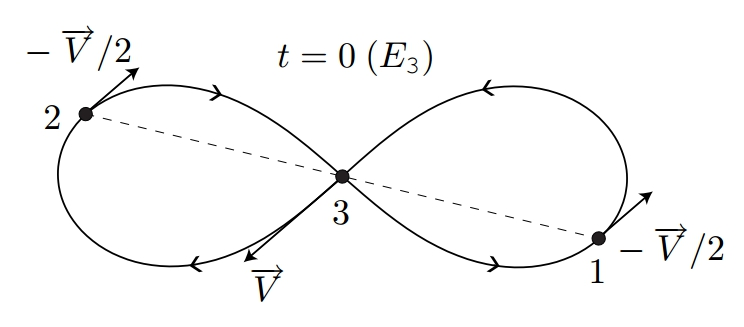
\includegraphics[width=7cm]{logo.jpg} \\ \vspace{0.3cm}Micha� D�browski}
\institute{17 X 2012}
\date{}
\title{{\sc Balet planetarny} \\ {\scriptsize Symulacje komputerowe w fizyce}}

\setbeamertemplate{footline}
{
\leavevmode
\hbox{
\begin{beamercolorbox}[wd=.9\paperwidth,ht=2.5ex,dp=1.125ex,right]{title in head/foot}
\end{beamercolorbox}
\begin{beamercolorbox}[wd=.1\paperwidth,ht=2.5ex,dp=1.125ex,center]{title in head/foot}
\usebeamerfont{author in head/foot}\insertframenumber/\inserttotalframenumber
\end{beamercolorbox}
}
\vskip0pt%
}

\begin{document}
\frame{
\titlepage
}

\frame{\frametitle{Ruch w polu grawitacyjnym}
\begin{block}{\sc Zadanie: Problem dw�ch cia�}
\begin{center}
\begin{itemize}
\item rozwi�za� (numerycznie) problem dw�ch cia�
\item $G=0.01$, $M=500$, $m=0.1$, $dt=0.001$, $N=30000$
\item warunki pocz�tkowe: $(x,y)=(2.0,0)$, $(p_x,p_y)=(0,0.1)$ \\
\item zastosowa� metody {\sc Eulera}, {\sc Verleta} i {\sc Leapfrog}
\end{itemize}
\end{center}
\end{block}
\vspace{0.2cm}
\begin{block}{\sc Zadanie{\Large \textcolor{yellow}{$^*$}}: �semka Chencinera}
\begin{center}
\begin{itemize}
\item rozwi�za� (numerycznie) problem trzech cia�
\item $G=1 $, $m_1=m_2=m_3=1$, $dt=0.001$, $N=20000$
\item warunki pocz�tkowe: \\
${\bf r_1}=-{\bf r_2}=(0.97000436,-0.24308753)$, ${\bf r_3}=(0,0)$ \\
${\bf v_3}=-2{\bf v_1}=-2{\bf v_2}=(0.93240737,0.86473146)$ \\
\item zastosowany algorytm: {\sc Leapfrog} (\textcolor{red}{animacja!})
\end{itemize}
\end{center}
\end{block}
}

\frame{\frametitle{Problem dw�ch cia� -- por�wnanie algorytm�w}
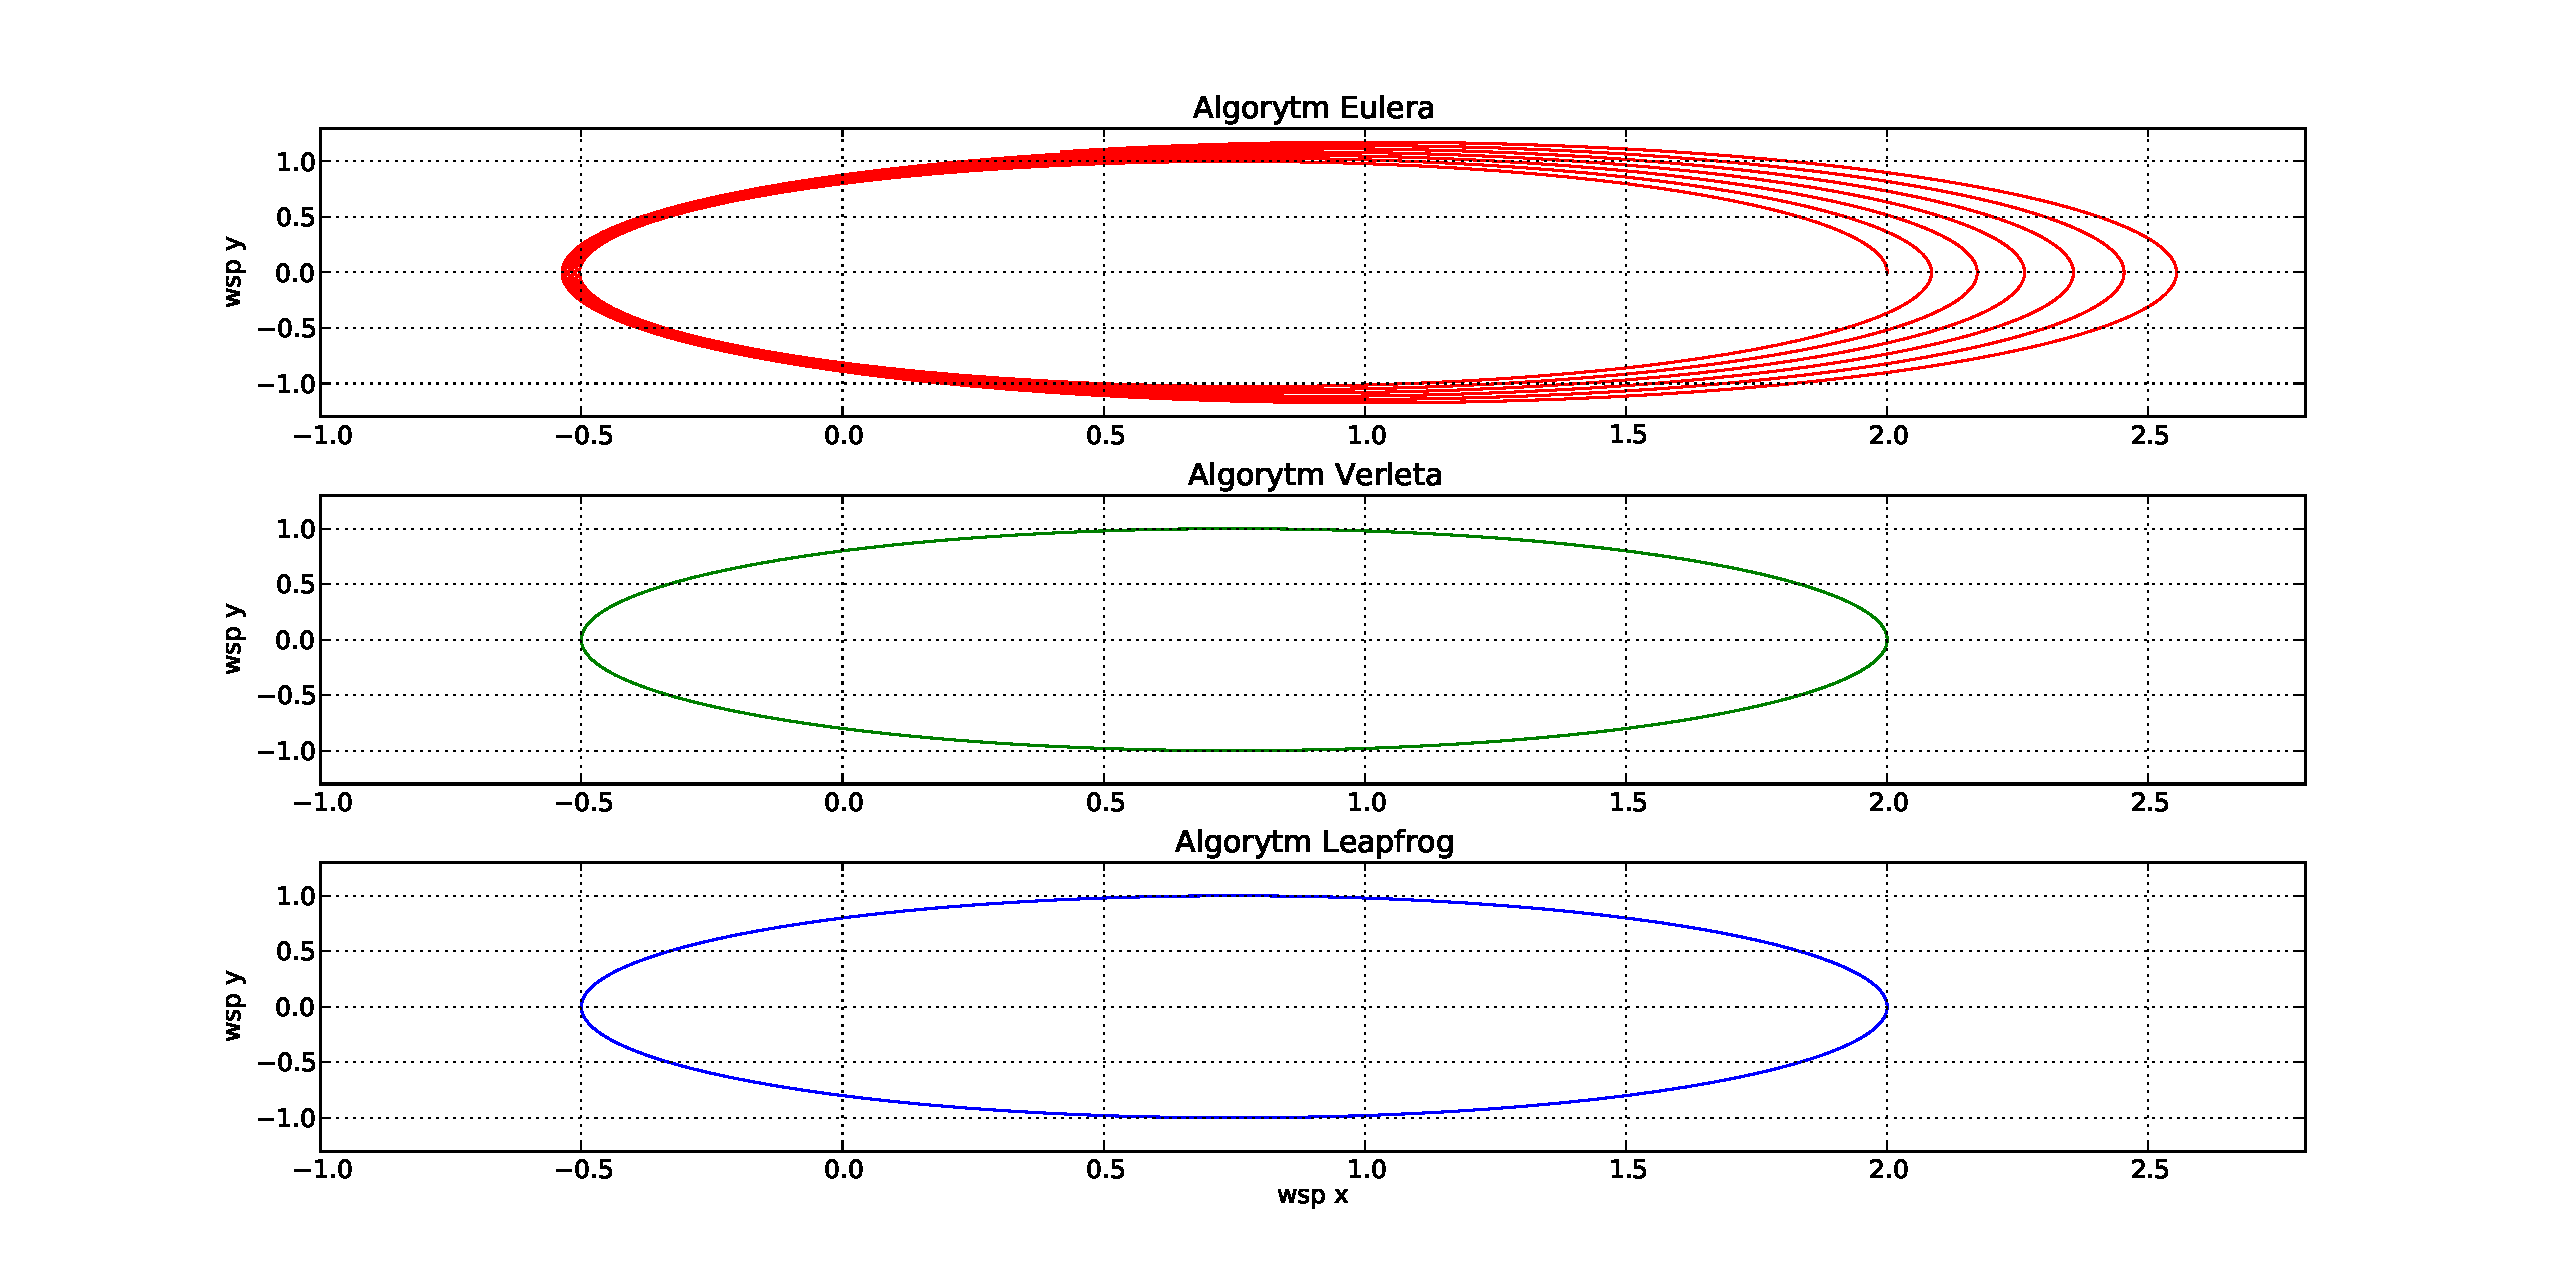
\includegraphics[width=12cm]{rys1.pdf}
\begin{itemize}
\item algorytm {\sc Eulera}: traci dok�adno�� w \textcolor{red}{peryhelium}
\item algorytm {\sc Verleta} i {\sc Leapfrog}: nierozr�nialne orbity
\end{itemize}
}

\frame{\frametitle{Problem dw�ch cia� -- por�wnanie algorytm�w}
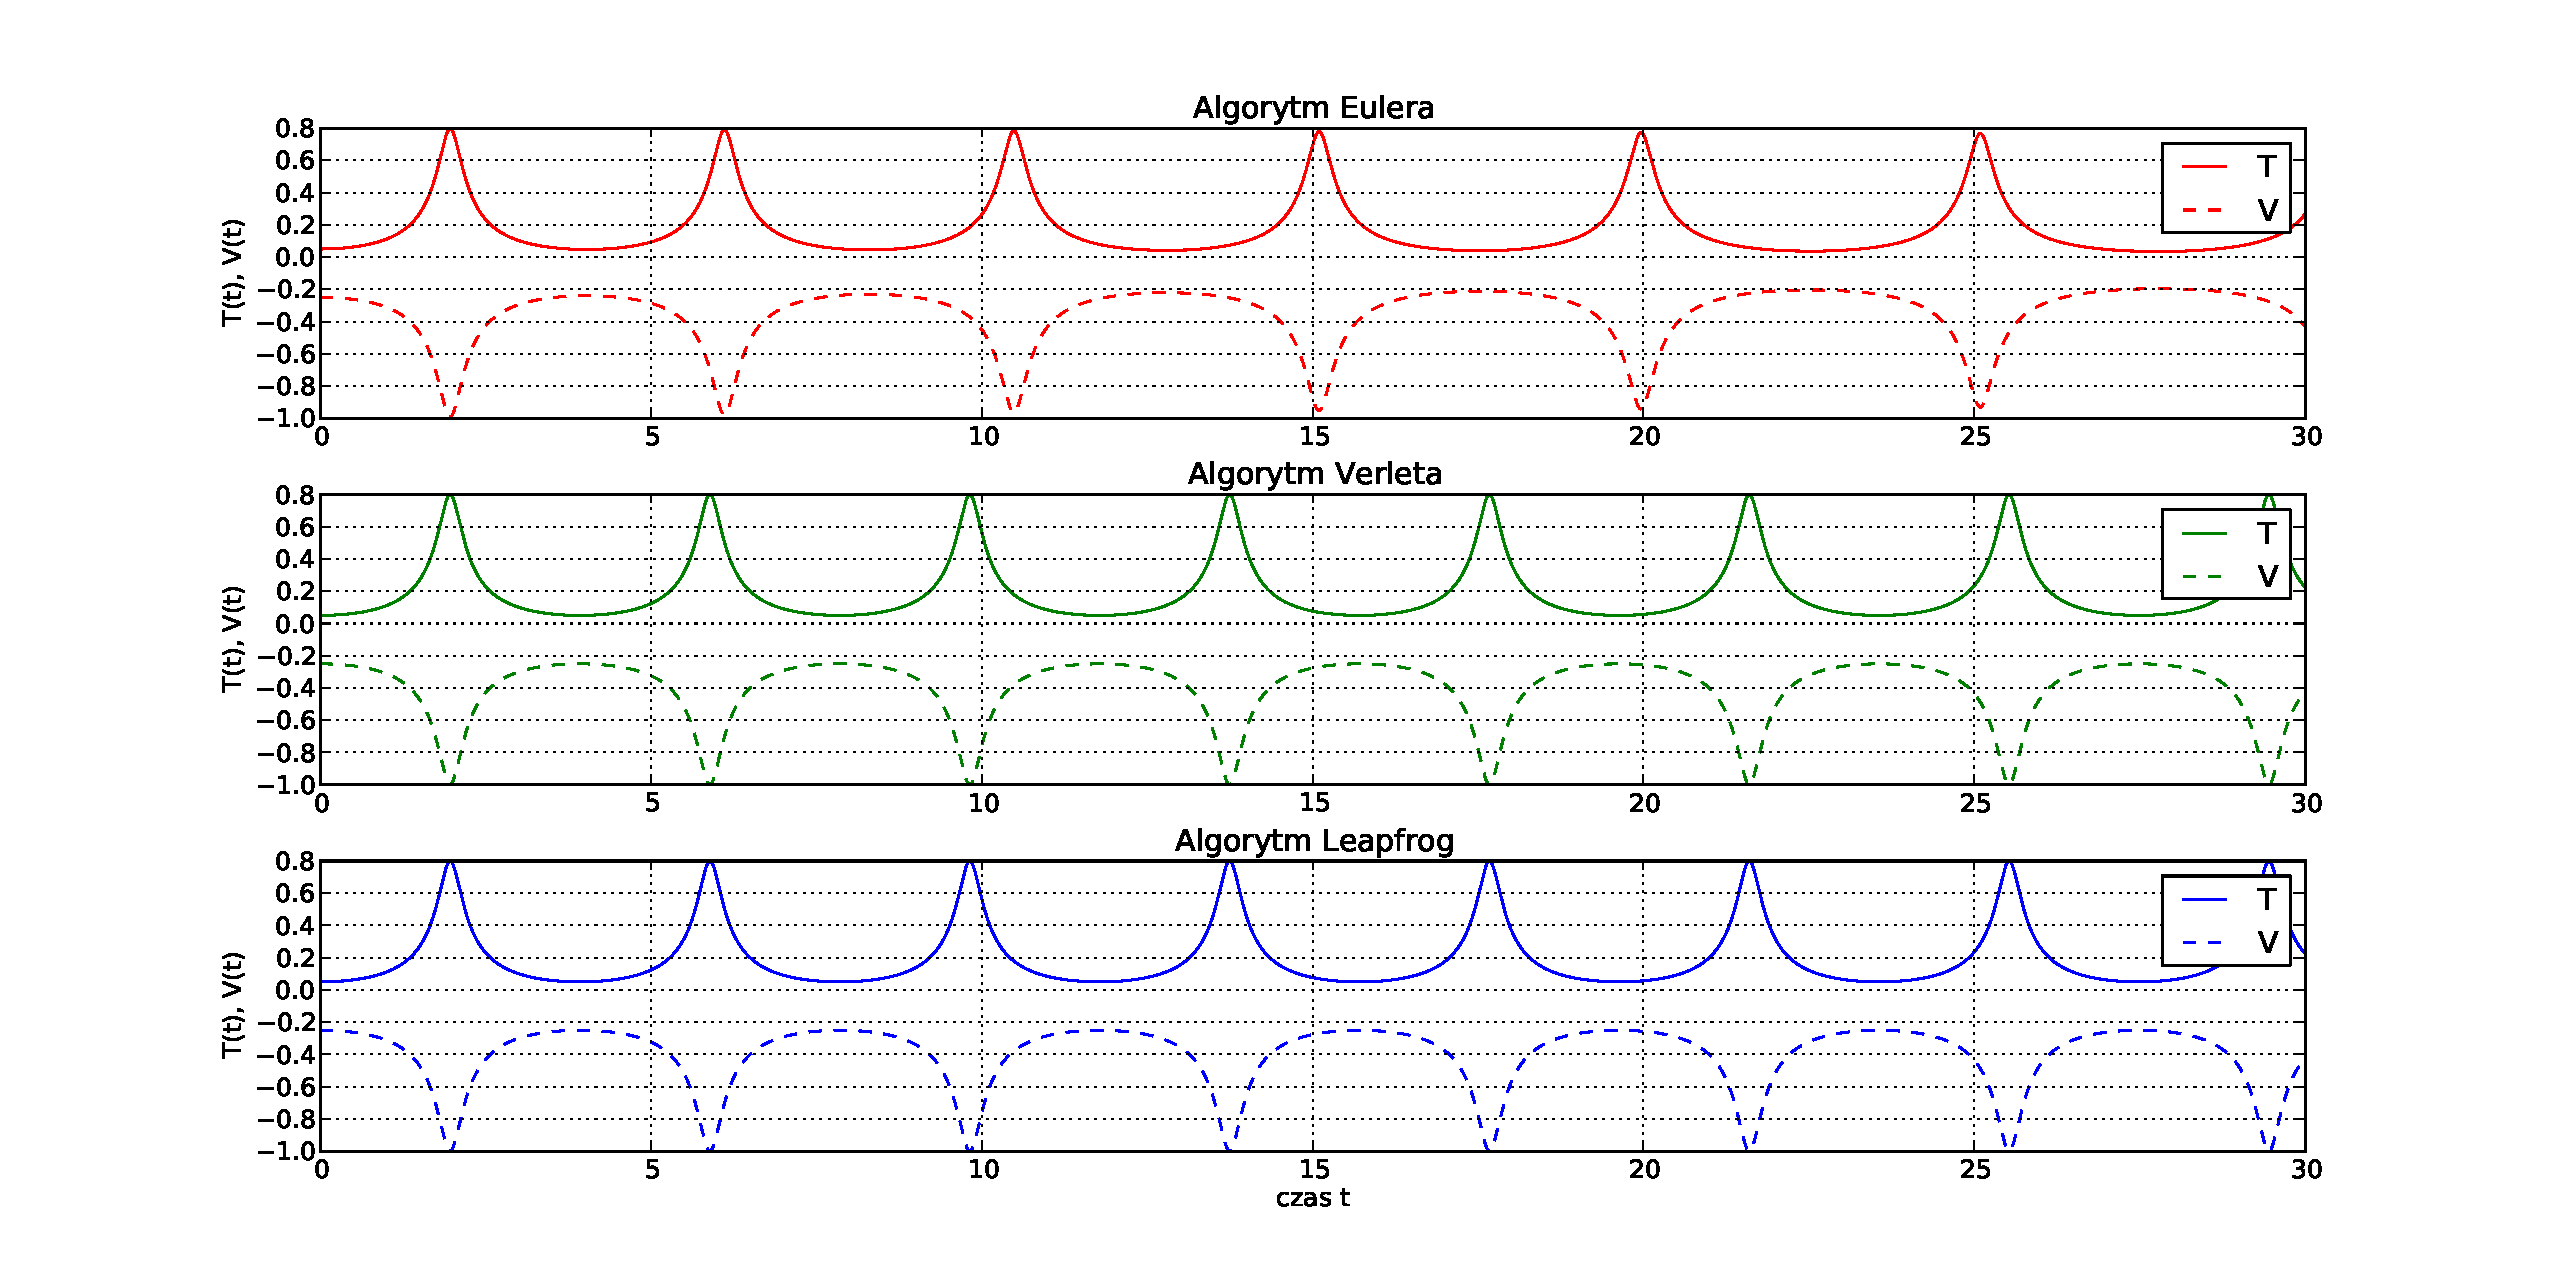
\includegraphics[width=12cm]{rys2.pdf}
\begin{itemize}
\item algorytm {\sc Eulera}: \textcolor{red}{wzrost okresu} ruchu po orbicie
\item algorytm {\sc Verleta} i {\sc Leapfrog}: sta�y okres ruchu
\end{itemize}
}

\frame{\frametitle{Problem dw�ch cia� -- por�wnanie algorytm�w}
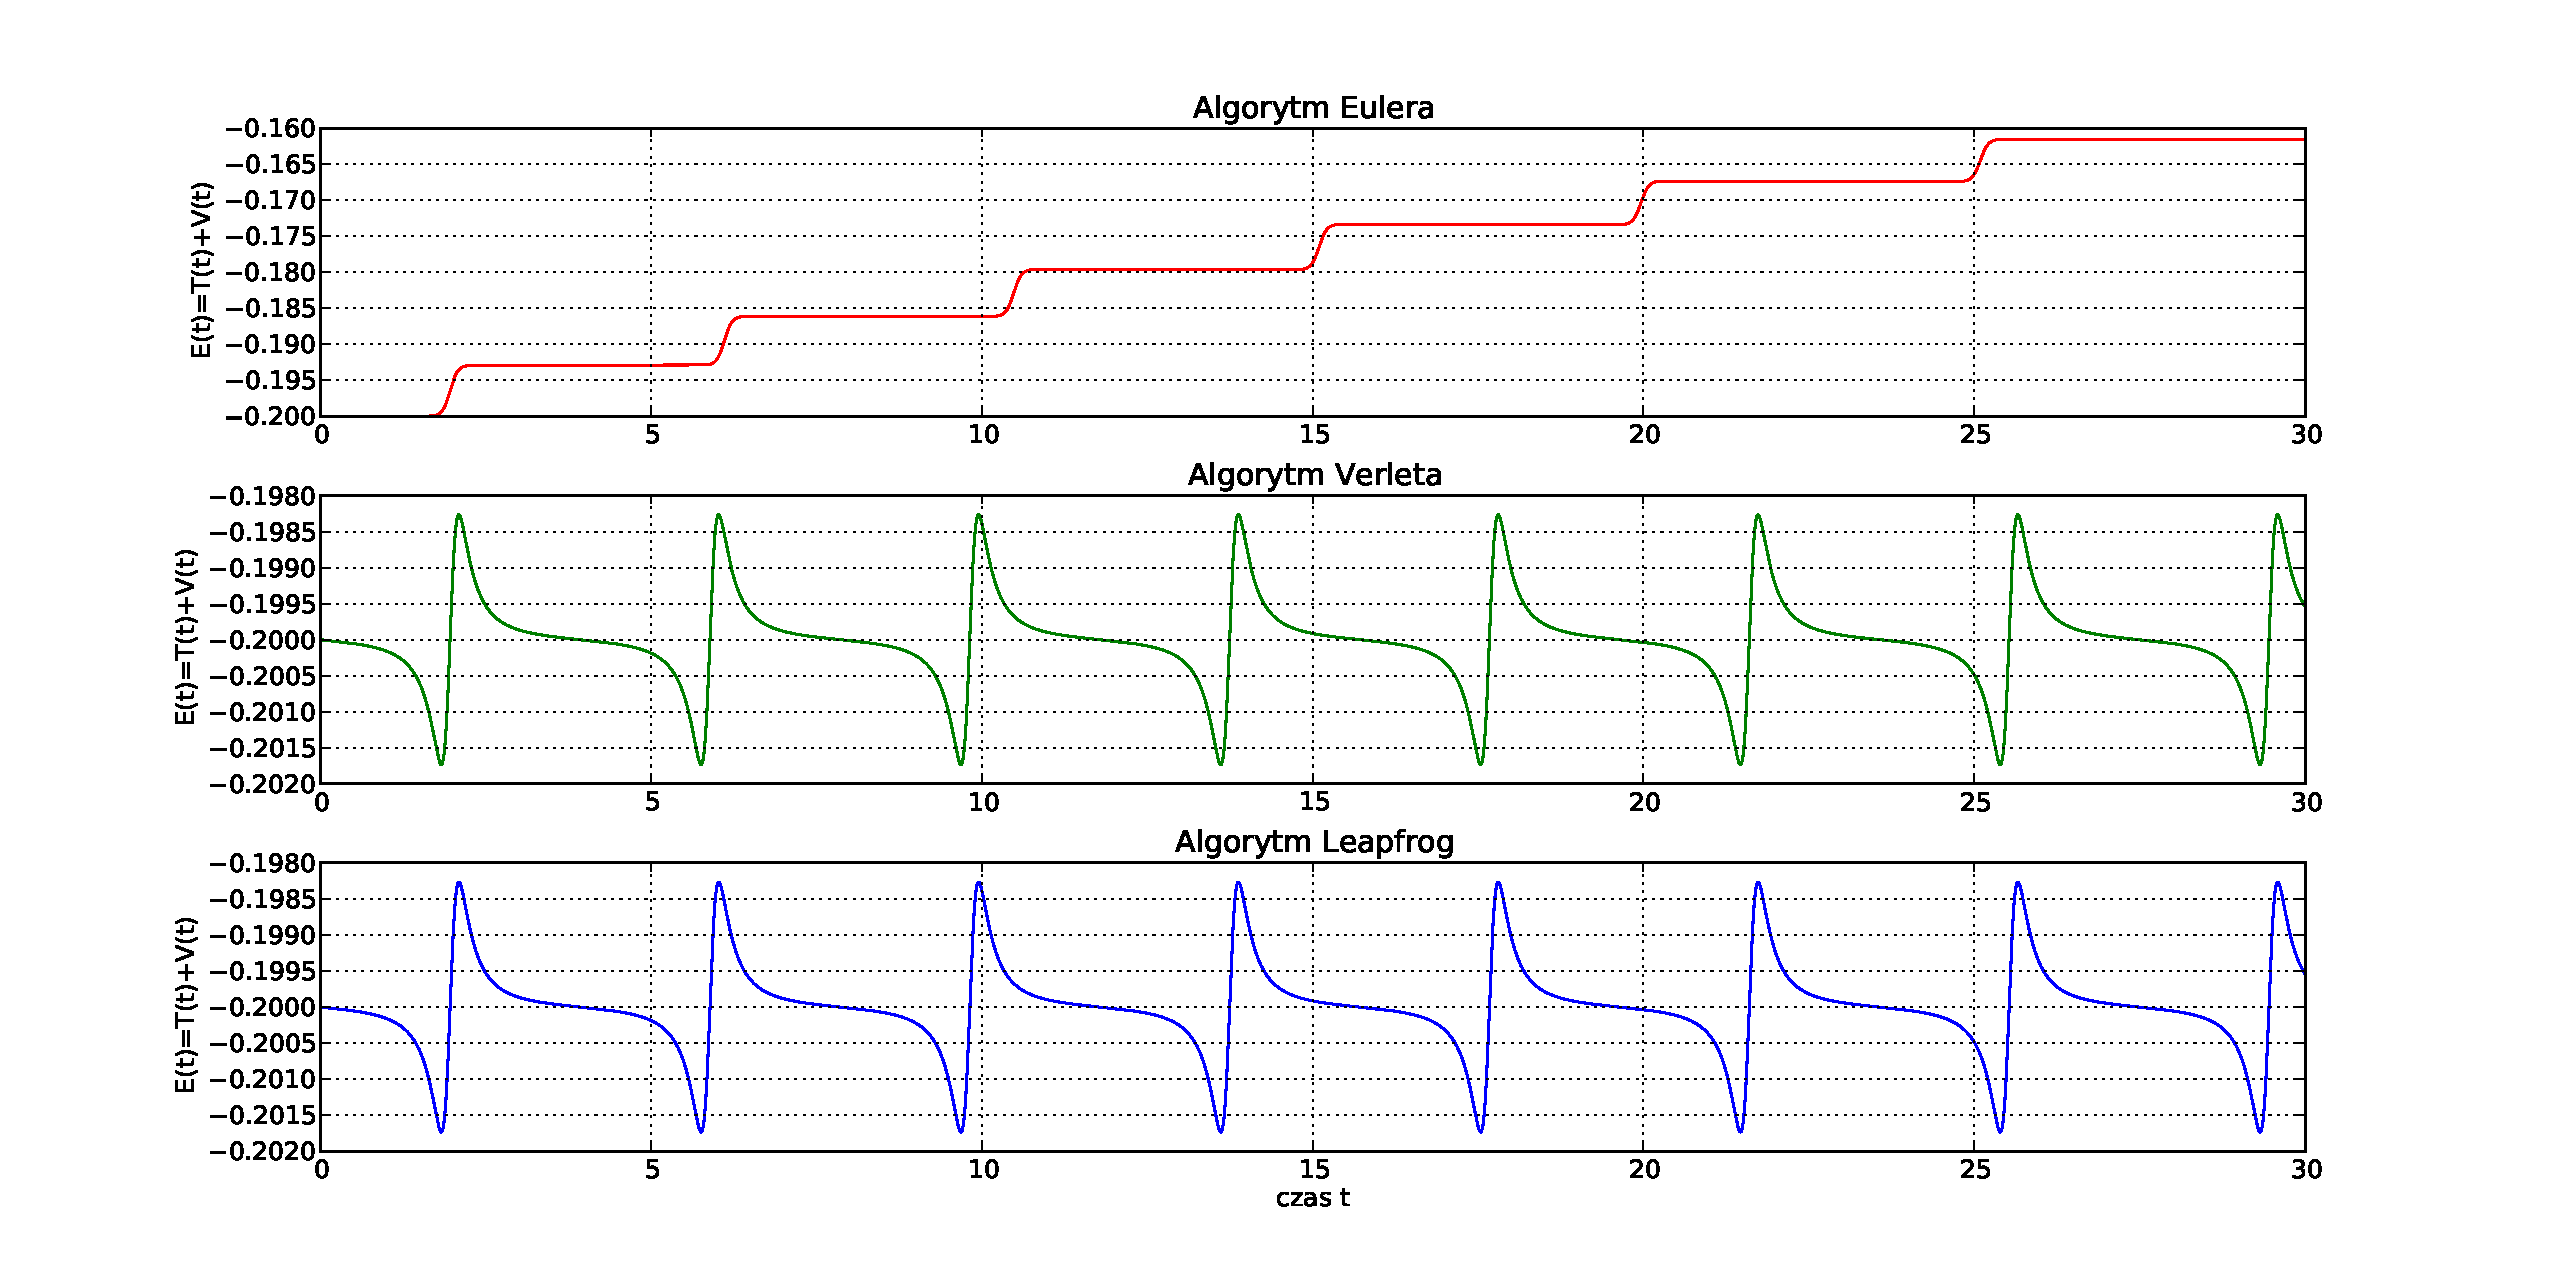
\includegraphics[width=12cm]{rys3.pdf}
\begin{itemize}
\item algorytm {\sc Eulera}: \textcolor{red}{energia} nieograniczenie \textcolor{red}{ro�nie}
\item algorytm {\sc Verleta} i {\sc Leapfrog}: energia oscyluje
\end{itemize}
}

\frame{\frametitle{Podsumowanie}
\begin{itemize}
\item algorytm {\sc Verleta} r�wnie dobry jak {\sc Leapfrog} \dots
\end{itemize}
\begin{figure}[H]
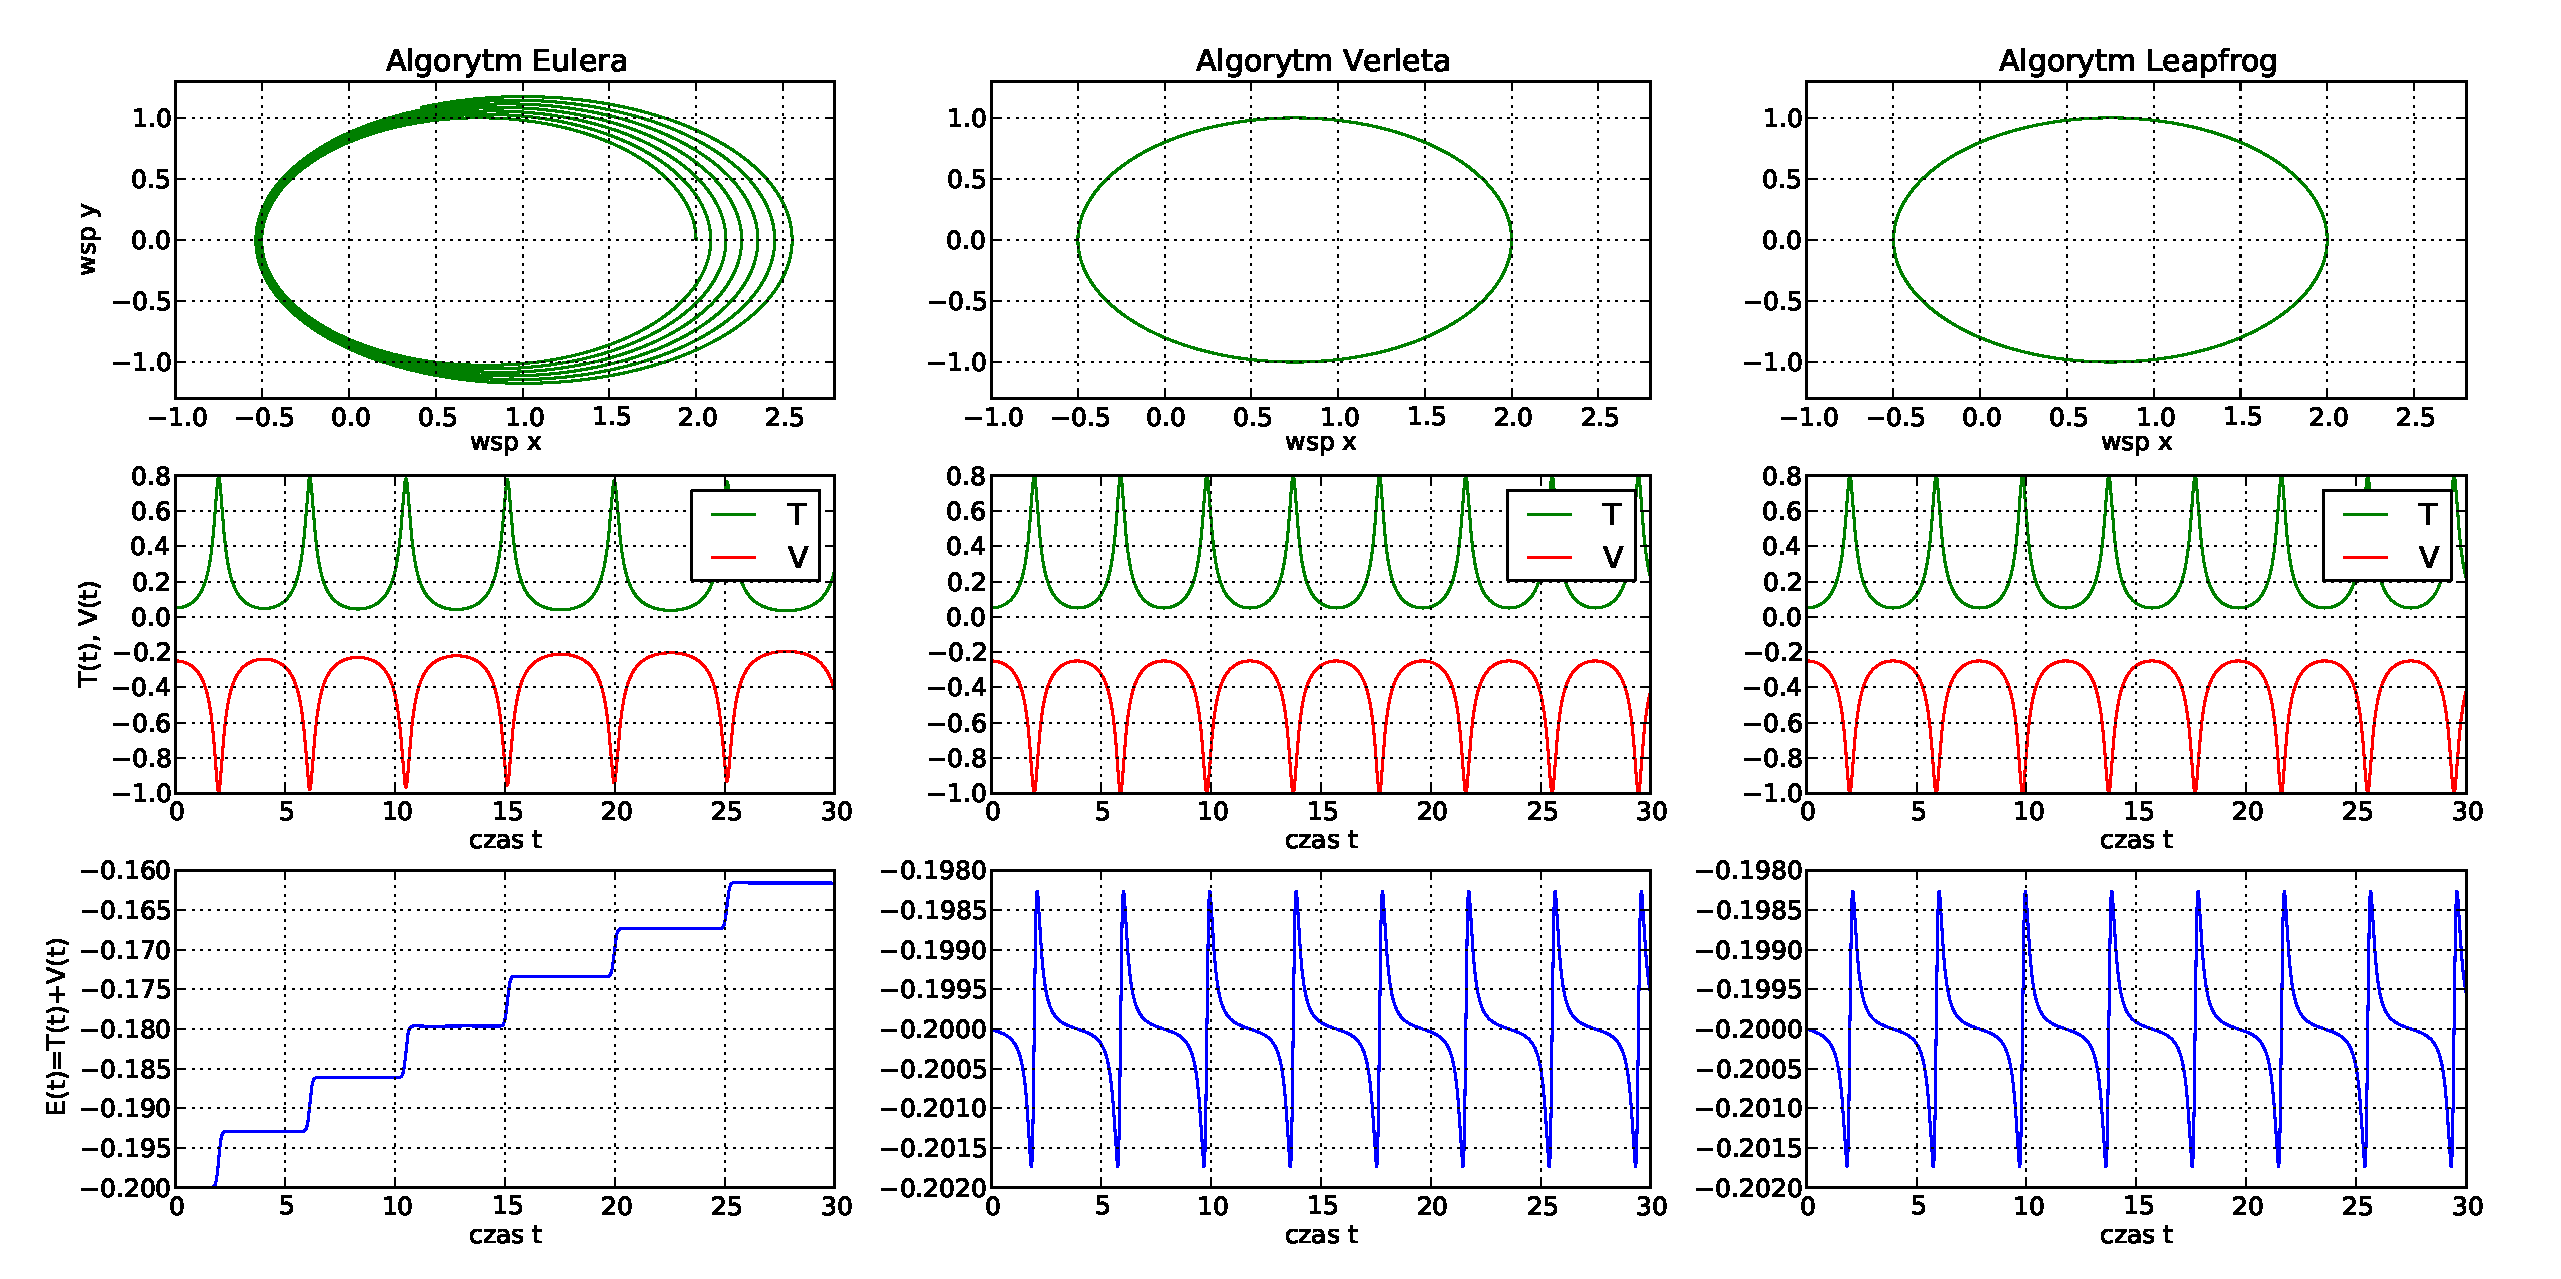
\includegraphics[width=11cm]{orbity.pdf}
\end{figure}
\begin{itemize}
\item \dots zatem czas na \textcolor{red}{animacj�} {\sc baletu planetarnego}!
\end{itemize}
}

\end{document}
